\chapter{回転するブロックを作る -- Tブロック}
\section{Tブロック}
今回はTブロックを作ります。Tブロックは、Tの字の形をしています。
Tブロックは、回転が必要なブロックです。回転するためには、ブロックの形を表す変数が必要です。
今回は、ブロックの形を方角と対応させて持つことにしますが、
\textbf{Tブロックの上の横棒が向いている方が方角になる}ようにします。また、カーソルの位置が
Tのくっついているところになるようにします。

\begin{figure}[h]
  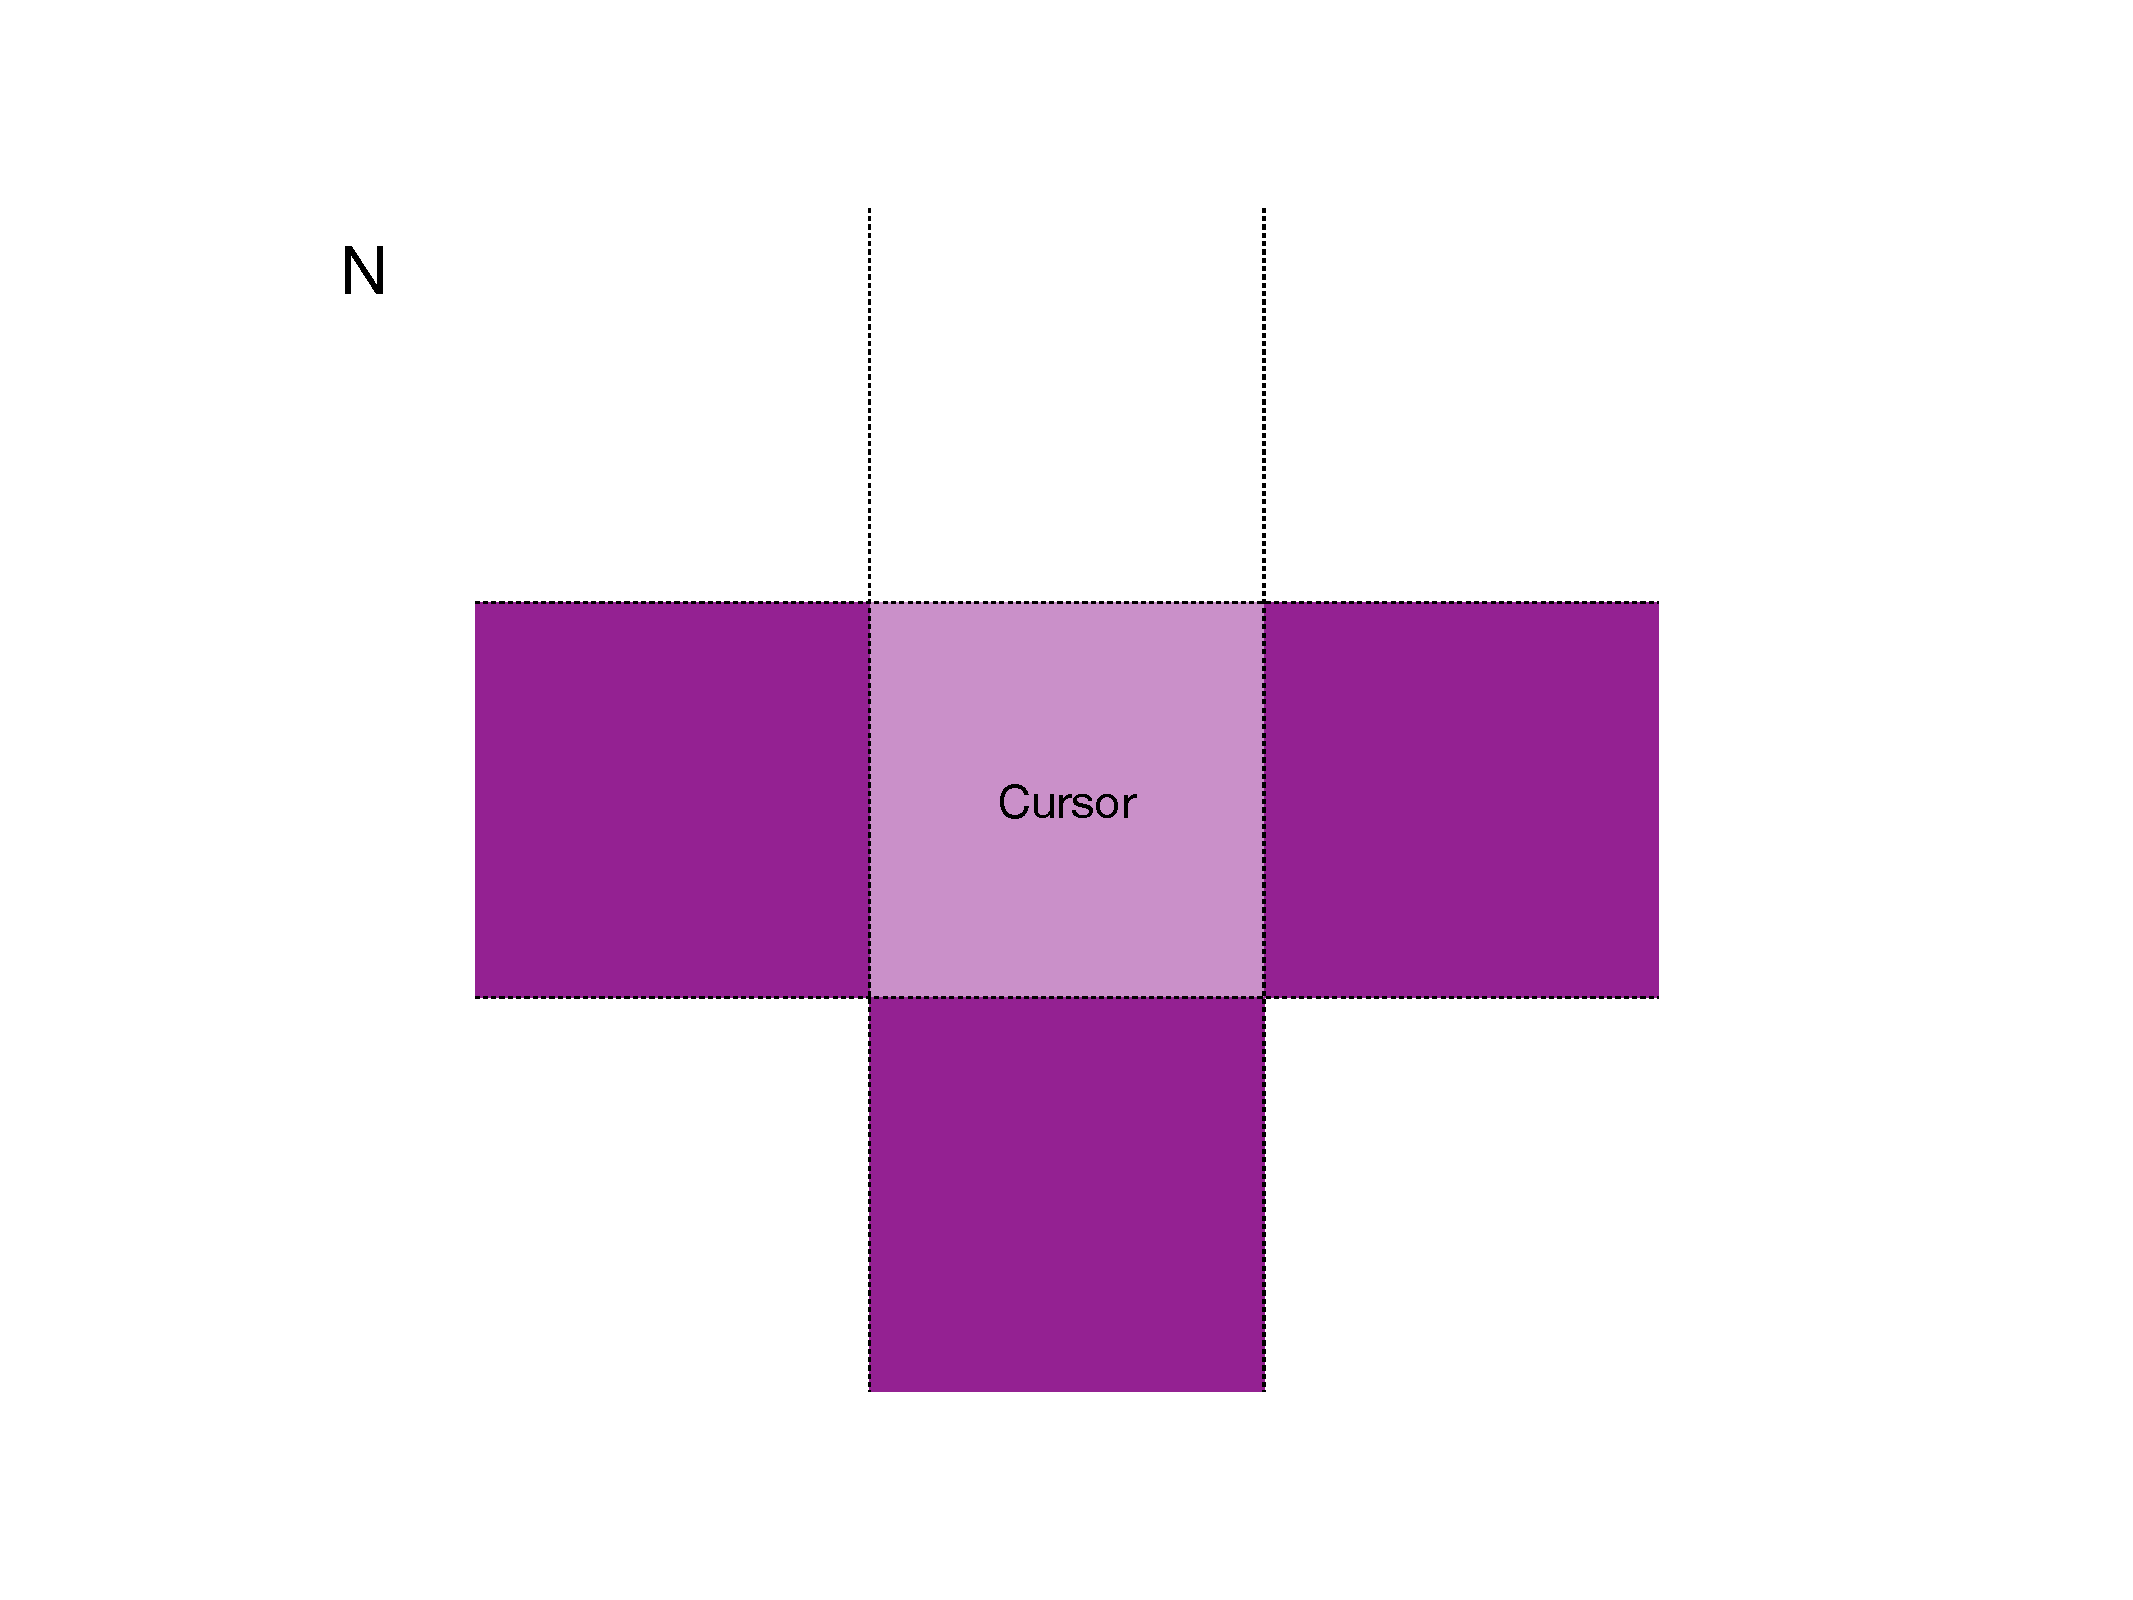
\includegraphics[width=70mm, page=1]{images/Blocks.pdf}
  \includegraphics[width=70mm, page=2]{images/Blocks.pdf}
  \includegraphics[width=70mm, page=3]{images/Blocks.pdf}
  \includegraphics[width=70mm, page=4]{images/Blocks.pdf}
  \caption{Tブロック}
\end{figure}

\newpage
\subsection{Tブロックのプログラム}

\lstinputlisting[caption={Tブロックのプログラム}, language=Python]{chapter7/ch7_1_1.py}

\newpage
\subsubsection{プログラミング豆知識}
回転系、周期系の変数の処理を楽に書きたいときは、それらを0から始まる数字の連番にすることと、
あまりが繰り返すことを利用すると上手く書けます。
\begin{lstlisting}[caption=方角を扱う,language=Python]
N=0
E=1
S=2
W=3
direction = N
direction = (direction + 1) % 4 # directionはE(1)になる
direction = (direction + 1) % 4 # directionはS(2)になる
direction = (direction + 1) % 4 # directionはW(3)になる
direction = (direction + 1) % 4 # directionはN(0)になる、3+1は4だが、4を4で割った余りは0なため
\end{lstlisting}
このように、Nから始まった方角がまたNに戻ってきます。

\subsection{Tブロックの描画}
Tブロックの描画は、Oブロックと同じように行います。
OブロックはBoardにblock\_infoを求められ、その情報をもとに描画していました。
でも、Tブロックもblock\_infoを持っていますから、Oブロックと同じように描画できます。
つまり、\textbf{Boardクラスは変更が必要ありません。オブジェクト指向の利点です。}
違うクラスであっても同じ名前で関数を設計すると、他のクラスから同じように扱えます。
でも中身自体は違うので、それぞれのブロックがそれぞれにあった情報を返すことができるのです。
こういう性質を「ポリモーフィズム/多態性」と言います
\footnote{厳密には違うんですがPythonにポリモーフィズムはあってないようなものなので教えるとしたらこうするしかないんです}。
では、main関数を変更して最初にTブロックを表示してみましょう。
\lstinputlisting[caption={テスト用にTブロックを表示}, language=Python]{chapter7/ch7_2_1.py}
できたら実行しましょう。表示だけで動かすとエラーになります。
\begin{figure}[h]
  \centering
  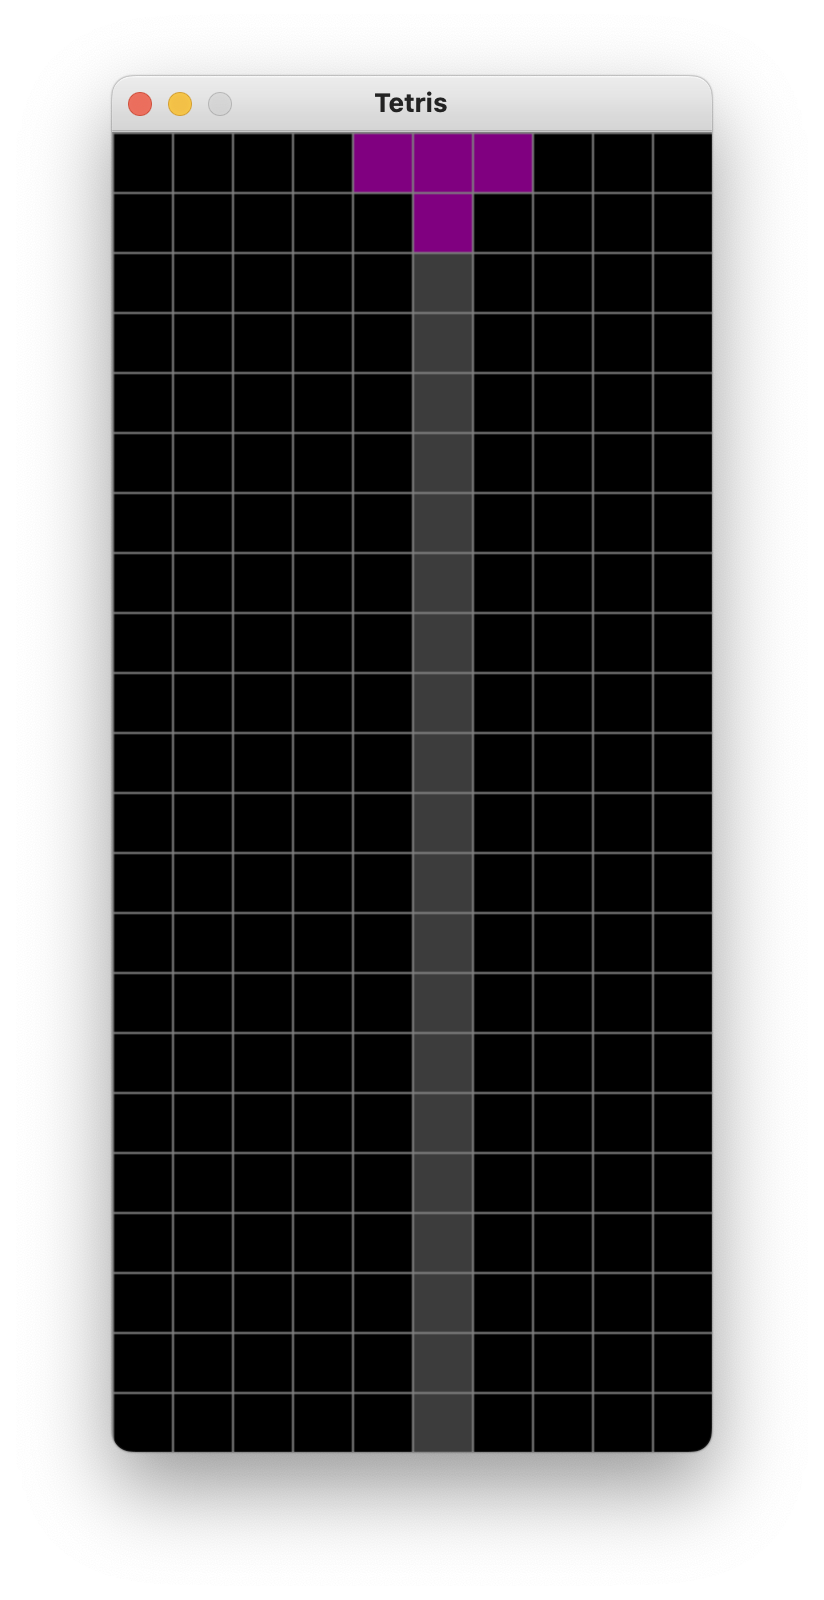
\includegraphics[width=50mm]{images/CH7_2.png}
  \caption{Tブロックの表示}
\end{figure}

\section{Tブロックを動かす}
なぜエラーになったのでしょうか?それは、Tブロックが動けるかどうかを判定する機能がないからです。
Oブロックは動けるかどうかを判定する機能を持っていましたが、Tブロックにはありません。
Boardはそのことを知らずにその関数を呼び出してしまったためエラーになります。
Tブロックにも動けるかどうかを判定する機能を追加しましょう。
\subsection{Tブロックに動けるかどうかを判定する機能を追加する}
TブロックにもOブロックと同じように、動けるかどうかを判定する機能を追加します。
\lstinputlisting[caption={Tブロックに動けるかどうかを判定する機能を追加}, language=Python]{chapter7/ch7_3_1.py}

\subsection{あれ、回転は?}
main関数でキー入力を受け取っていますので、main関数を実行して回転キーを設定しましょう。

\lstinputlisting[caption={main関数で回転する}, language=Python]{chapter7/ch7_4_1.py}
書き終えたら実行してみましょう。ひとまずお疲れ様でした。でも、まだ終わりではありません。
\begin{figure}[h]
  \centering
  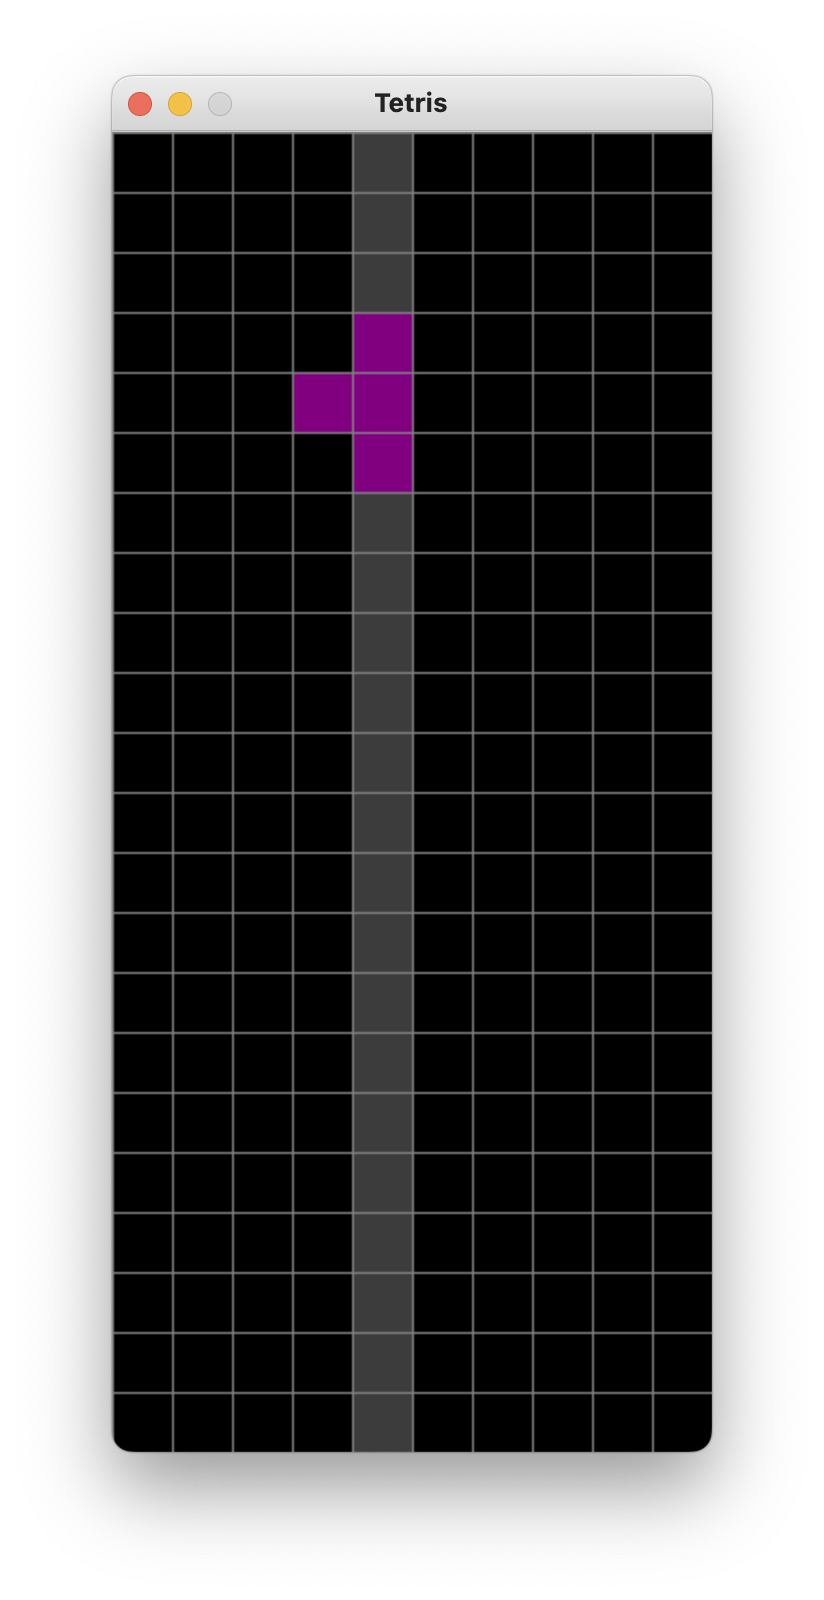
\includegraphics[width=50mm]{images/CH7_4.png}
  \caption{Tブロックの回転}
\end{figure}

回転によりはみ出してしまうことがありますね。これは移動と同じで回転できない状況があるのに、それを検知できずに回転しているからです。

\subsubsection{Q: この教材、いきあたりばったりで作ってないですか?}
多くのメンターさんが共感してくれると思いますが、
基本的にプログラムは一発で動きません。さらに残酷なことに、頑張って書いた時ほど、動かないものです。
ここまできたみなさんには、同じプログラマとして、「せっかく頑張ったのになんでやねん」というこのガッカリ感を
味わってみて欲しいです。

実行する前にこうなることが予期できた人は素晴らしいです。ぜひ、次回以降もこのような予測をしていってください。

\section{回転できるか判定する関数をつくる}
それでは、回転について判定する関数を作ってみましょう。
いくつか方法が考えられますが、今回は、回転した後の座標を計算して、その座標が盤面と衝突しないかどうかを判定する方法を取ります。
\subsection{回転できるか判定する関数をつくる}
以下のように書いてみましょう。戻り値はbool型、すなわちTrueかFalseです。
可能だと分かったらその時点でreturn True、逆に不可能だと分かったらreturn Falseします。
\lstinputlisting[caption={回転できるか判定する関数をつくる}, language=Python]{chapter7/ch7_5_1.py}
ちなみに、もっと賢い方法を思いついた人は、それを書いて試してみましょう。
この教材では直感的な方法をとっています。

次に、\textbf{判定をしてから回転する}部分を作ります。
今回も前回同様に、Boardクラスがブロックの回転する関数を提供します。
\subsection{Boardクラスに回転する関数をつくる}
\lstinputlisting[caption={Boardクラスに回転する関数をつくる}, language=Python]{chapter7/ch7_5_2.py}
これで回転できる時に回転する、機能が完成しました。
最後に、main関数を変更しましょう。
\subsection{main関数を変更する}
\lstinputlisting[caption={main関数を変更する}, language=Python]{chapter7/ch7_5_3.py}
実行すると、Tブロックが正しく回転するようになるはずです。
うまくいかない場合はcan\_rotateが大体間違っていると思うので、先生と相談してください。

\subsubsection{コラム: if \_\_name\_\_ == "\_\_main\_\_"について}
Swimmyの教材には書いていませんが、Pythonには\_\_name\_\_という変数があらかじめ使えます。
もちろん変数なのでprintが可能です。
\begin{lstlisting}[caption=\_\_name\_\_の使い方,language=Python]
print(__name__)
\end{lstlisting}
これを実行すると、\_\_main\_\_と表示されます。これは、このファイルが直接実行されたときに\_\_main\_\_になるということです。
Pythonファイルには、実行する方法が2度あります。
\begin{itemize}
  \item 直接実行する
  \item importして使う
\end{itemize}
importされた時には、\_\_name\_\_はファイル名になります。
import pygameをしたときに
\begin{verbatim}
pygame 2.0.1 (SDL 2.0.14, Python 3.8.3)
Hello from the pygame community. https://www.pygame.org/contribute.html
\end{verbatim}
こんな表示を見たことはありませんか?
おそらく、pygameのファイルにはこんなのが書いてあるはずです
\begin{lstlisting}[caption=pygameのファイルの一部,language=Python]
  print("pygame 2.0.1 (SDL 2.0.14, Python 3.8.3)")
  print("Hello from the pygame community. https://www.pygame.org/contribute.html")
\end{lstlisting}
使い道はかなり限定されていますが、
\begin{itemize}
  \item このファイルが間違ってimportされた時に警告を出したい
  \item importして使って欲しいので直接実行された時はエラーを出したい
  \item バージョンを表示したり、著作権表示をしたい
\end{itemize}
こんな時に使われている傾向があります。
せっかくなので、自分のファイルにも書いてみてください。
\lstinputlisting[language=Python]{chapter7/ch7_5_4.py}
import tetrisのあたりでprintが実行され、自分の名前が出てくるはずです。

\section{まとめ}
今回はTブロックを作りました。TブロックはOブロックと違い、回転が必要なブロックです。
そのため、回転できるかどうかを判定する機能を追加しました。